% =============================================================================
%  Selective State-Space Models for TESS Exoplanet Vetting from Long Light Curves
%  IEEE conference format (IEEEtran, two columns).
%
%  Target venues: IEEE Latin America Transactions / IEEE conference,
%  NeurIPS "Machine Learning and the Physical Sciences" workshop (port style).
%
%  Font note: lmodern is loaded so the PDF embeds Type 1 outlines (no Type 3
%  bitmaps) and text/ligatures extract correctly. For a Times camera-ready,
%  replace lmodern with: \usepackage{newtxtext}\usepackage{newtxmath}.
% =============================================================================
\documentclass[conference]{IEEEtran}

\usepackage[utf8]{inputenc}
\usepackage[T1]{fontenc}
\usepackage{lmodern}        % Type 1 outlines (no Type 3 bitmaps)
\input{glyphtounicode}
\pdfgentounicode=1          % correct ToUnicode for ligatures (fi, ff, ...)

\usepackage{cite}
\usepackage{amsmath,amssymb,amsfonts}
\usepackage{graphicx}
\usepackage{booktabs}
\usepackage{xcolor}
\usepackage{textcomp}
\usepackage[hidelinks]{hyperref}
\usepackage{xurl}
\usepackage[caption=false,font=footnotesize]{subfig}
\usepackage{balance}

\begin{document}

\title{Selective State-Space Models for TESS Exoplanet Vetting from Long Light
Curves}

\author{
\IEEEauthorblockN{Jos\'e Fabi\'an Zumbado Ruiz and Jeremmy Aguilar Villanueva}
\IEEEauthorblockA{School of Computing, Instituto Tecnol\'ogico de Costa Rica\\
Cartago, Costa Rica\\
\{jzumbado, jaguilar\}@estudiantec.cr}
}

\maketitle

% -----------------------------------------------------------------------------
\begin{abstract}
Selective state-space models such as Mamba process long sequences in linear time,
but their usefulness for exoplanet vetting from TESS light curves has not been
evaluated. We present a controlled feasibility study for confirmed-planet (CP)
versus false-positive (FP) vetting of TESS Objects of Interest using complete
global light curves of length $L=18{,}000$. On 1{,}576 labelled TOIs under a sealed
TIC-level split, a compact Mamba model reaches AUC-ROC $0.806$ (95\% bootstrap CI
$[0.747,0.857]$), compared with $0.604$ for an AstroNet-style single-branch CNN and
$0.605$ for catalog logistic regression. The Mamba--CNN gap is statistically
significant (DeLong $p=3.7\times10^{-8}$; paired-bootstrap $\Delta$AUC CI
$[+0.13,+0.28]$). A larger AstroNet-style dual-branch baseline lands between the CNN
and Mamba. Attribution methods localize Mamba's evidence to transit dips in true
positives. We frame this as the first controlled feasibility evidence for selective
state-space modeling in this specific TESS CP/FP vetting setting, not as a
state-of-the-art vetting catalog.
\end{abstract}

\begin{IEEEkeywords}
exoplanet vetting, TESS, Mamba, state-space models, light curves, reproducibility
\end{IEEEkeywords}

% =============================================================================
\section{Introduction}

The Transiting Exoplanet Survey Satellite (TESS) observes $>$200{,}000 stars at
2-minute cadence, producing $\sim$18{,}000 photometric measurements per star per
$\sim$27-day sector. Transit signals are shallow ($\sim$0.01--1\% flux dips) and
morphologically degenerate with eclipsing binaries and instrumental systematics,
which makes large-scale \emph{vetting}---deciding whether an already-detected
candidate is a confirmed planet (CP) or a false positive (FP)---a central
bottleneck. Our task is vetting, not detection: NASA's pipeline performs the
Box-Least-Squares search; we evaluate light-curve models and catalog-feature
baselines on the resulting TESS Objects of Interest (TOIs). Catalog metadata
(orbital period, transit depth, epoch, stellar magnitude) is used only where it is
part of the model definition---as logistic-regression features or for phase-folding
the local view---not as a side input to the sequence models; using it is therefore
not leakage in this vetting setting, consistent with established
practice~\cite{shallue2018,valizadegan2022}.

State-of-the-art vetting is built on 1D convolutional networks
\cite{shallue2018,valizadegan2022,exominerpp,dartvetter}. A shallow single-branch
CNN, however, sees the curve as a bag of local patches: stacking a few
AstroNet-style blocks yields an effective receptive field of only $\sim$80 cadences
($\sim$20 minutes of observation), far shorter than the multi-day spacing between
transits in a sector (deeper or dilated stacks widen this, at additional cost).
Transformers would model the full sequence but at $O(L^2)$ cost---prohibitive for
$L=18{,}000$ on commodity hardware. Selective state-space models
(Mamba~\cite{gu2023mamba}) propagate an input-dependent latent state across the
whole sequence in $O(L)$ time and constant memory, which is exactly the regime of
long photometric series. To our knowledge, Mamba has not been evaluated for
CP/FP vetting of TESS TOIs on the complete global light curve.

\textbf{Contributions.} (i) The first controlled comparison of a selective
state-space model against tabular and convolutional baselines for TESS TOI
vetting on full 18{,}000-cadence global curves, under one sealed star-level split.
(ii) A statistically grounded evaluation---bootstrap confidence intervals for
AUC-ROC and DeLong tests for paired AUC differences---rather than point
estimates alone. (iii) A close AstroNet-inspired dual-branch baseline adapted to
the TESS setting as a strong upper-reference, plus a clearly labelled
negative ablation (a naive Mamba$+$CNN late-fusion). (iv) Explainability
(saliency, integrated gradients, occlusion) localizing the model's evidence to the
transit dips. We deliberately make a \emph{narrow, defensible} claim: under small
data and a 4\,GB GPU, Mamba extracts temporal signal that tabular features and a
single-branch CNN miss; we do not claim a new vetting state of the art.

% =============================================================================
\section{Related Work}

Deep learning for transit vetting began with AstroNet~\cite{shallue2018}, a
dual-branch (global$+$local) CNN for Kepler that ranked candidates above
classical features. ExoMiner~\cite{valizadegan2022} extended this with
expert-diagnostic inputs and validated hundreds of new exoplanets;
ExoMiner++~\cite{exominerpp} ports the approach to TESS 2-minute data with
Kepler-to-TESS transfer learning and additional diagnostics (periodograms,
difference images, spacecraft attitude). For TESS specifically,
Yu et al.~\cite{yu2019} performed automated triage/vetting with CNNs, reporting an
average precision of 69.3\% in the vetting setting. Lighter, easier-to-replicate
CNNs such as DART-Vetter~\cite{dartvetter} continue this line, and broader
machine-learning validation frameworks have been applied to candidate validation
\cite{armstrong2020}. These systems are strong and, in several cases, rely on
large training sets and/or transfer learning; we therefore do not position our
work as competing for state of the art.

Mamba~\cite{gu2023mamba} introduced selective state-space sequence modeling with
linear-time scaling and a hardware-aware scan. It has been applied across
language, audio and vision, but---to our knowledge---not to CP/FP vetting of TESS
TOIs from the full global light curve. That gap is the niche this study addresses
with a controlled, low-cost experimental comparison.

% =============================================================================
\section{Data and Problem Setup}

\textbf{Sources.} Labels come from the NASA Exoplanet Archive TOI
catalog~\cite{toi}; light curves are the PDCSAP\_FLUX series retrieved from
MAST~\cite{mast} via \texttt{lightkurve}~\cite{lightkurve}. We define a binary
task: confirmed planets (CP) as the positive class and false positives (FP) as the
negative class, yielding 1{,}576 labelled TOIs after quality filtering (603 CP /
973 FP, a $\sim$1{:}1.6 imbalance).

\textbf{Preprocessing.} Each curve is normalized by its own median (no global
dataset statistics, to avoid scale leakage across splits); NaNs and
poor-quality cadences are masked/interpolated; all curves are fixed to
$L=18{,}000$ by truncation/padding. The \emph{global view} is this full series.
For the dual-branch ablations we additionally build a \emph{local view} by
phase-folding on the catalog $(P, T_0)$, restricting to $|\phi-0.5|\le 2.5\,D/P$
and binning to 201 points; TOIs with missing/degenerate ephemerides or
$P>27.4$\,d (one sector) are excluded from the local-view subset.

\textbf{Sealed, star-level split.} A star may appear in several TESS sectors;
splitting at the observation level would place the same TIC in train and test
(severe leakage). We split at the \emph{TIC} level, 70/15/15, preserving class
balance, and we evaluate the test set \emph{once} per model. The local-view
subset is a strict subset of the same split (no TIC changes fold), so its
test set ($N=210$) is smaller than the global test set ($N=237$); the two are not
directly comparable and we report paired statistics only on shared samples.
Table~\ref{tab:splits} gives the counts.

\begin{table}[!t]
\caption{Star-level (TIC) splits. The local-view subset is a strict subset of the
global split, filtered to TOIs with usable ephemerides ($P\le27.4$\,d).}
\label{tab:splits}
\centering
\footnotesize
\begin{tabular}{lrlrl}
\toprule
Split & Global $N$ & CP/FP & Local-view $N$ & CP/FP \\
\midrule
train & 1103 & 422/681 & 985 & 376/609 \\
val   & 236  & 90/146  & 211 & 77/134 \\
test (sealed) & 237 & 91/146 & 210 & 78/132 \\
\midrule
total & 1576 & 603/973 & 1406 & 531/875 \\
\bottomrule
\end{tabular}
\end{table}

% =============================================================================
\section{Models}

We evaluate a ladder of models in which each rung adds one design variable, so
each AUC delta is attributable to a concrete component.

\textbf{Baselines.}
(1) \emph{Stratified prior}: predicts the class prior; an empirical floor
(AUC $=0.5$).
(2) \emph{Catalog logistic regression}: $\ell_2$-regularized logistic regression on
\emph{only} three catalog features (orbital period, transit depth, stellar
magnitude), standardized with statistics fit on train only and class-balanced.
Epoch ($T_0$) and transit duration ($D$) are \emph{not} used by this baseline;
they serve only to build the phase-folded local view. It answers
whether catalog metadata alone separates CP from FP.
(3) \emph{CNN single-branch} (AstroNet-inspired, global view only): four
\texttt{Conv1d}$\,\to\,$BN$\,\to\,$ReLU$\,\to\,$MaxPool blocks
(channels $16{\to}32{\to}64{\to}128$), global average pooling, and a small MLP head
(62{,}881 parameters).

\textbf{Mamba single-view (focus model).} A linear embedding
($1{\to}d_{\text{model}}{=}64$), four residual Mamba blocks
($d_{\text{state}}{=}16$, $d_{\text{conv}}{=}4$, expand$=2$) with LayerNorm, global
average pooling, and a linear classifier (131{,}393 parameters). Gradient clipping
(\texttt{max\_norm}$=1.0$) is essential: without it the model diverges to NaN on the
long sequences. The state recursion
$h_t=\bar{\mathbf{A}}_t h_{t-1}+\bar{\mathbf{B}}_t x_t,\; y_t=\mathbf{C}_t h_t$,
with input-dependent $(\bar{\mathbf{A}},\bar{\mathbf{B}},\mathbf{C})$, lets the
model integrate evidence across all 18{,}000 cadences and selectively down-weight
noisy gaps.

\textbf{Dual-branch ablations (local-view subset).}
(4) \emph{AstroNet multibranch}: a close AstroNet-inspired dual-branch baseline
following Shallue \& Vanderburg~\cite{shallue2018}, adapted to TESS---a deep global
branch (five double-conv blocks, $16{\to}256$), a shallow local branch,
concatenation, and a four-layer FC head (1{,}338{,}081 parameters). Because the
original \texttt{Flatten} over $L=18{,}000$ is infeasible, we use adaptive average
pooling on the global branch; the model needs batch size 8, FP16 and gradient
checkpointing to fit in 4\,GB. (5) \emph{ExoMamba V1 (negative ablation)}: a naive
late-concat fusion of the Mamba global encoder with a small 3-block local CNN
($\sim$153K parameters).

% =============================================================================
\section{Experimental Protocol}

All neural models are trained with class-weighted binary cross-entropy and
AdamW, with early stopping on validation AUC-ROC; the test set is untouched
during development. We do not use $k$-fold cross-validation: a single Mamba run
takes $\sim$1\,h on an RTX 3050 (4\,GB), so $k{=}5$ over a hyperparameter sweep
would cost $\sim$100 GPU-hours. As a statistical proxy we report \emph{multi-seed}
variability---five seeds for Mamba single-view, three for the dual-branch
ablations---and a probability-averaged \emph{ensemble} per model family. The Mamba
hyperparameters were chosen by a small structured search on validation
(learning rate $1.5\times10^{-3}$; $d_{\text{state}}{=}16$; patience 10), not an
automated tuner, again for cost.

\textbf{Inference statistics.} On the sealed test set we report 95\% bootstrap
confidence intervals (2{,}000 stratified resamples) for AUC-ROC in
Table~\ref{tab:main}; AUC-PR is listed as a point estimate, and its bootstrap CI is
computed identically and included in the released statistics file.
For paired model comparisons on shared samples we report DeLong's
test~\cite{delong1988} (fast formulation~\cite{sun2014}) for the AUC difference,
together with a stratified paired-bootstrap CI for $\Delta$AUC.

% =============================================================================
\section{Results}

\subsection{Main comparison}

Table~\ref{tab:main} reports test metrics with bootstrap CIs.
Mamba single-view reaches AUC-ROC $0.806$ (ensemble) and $0.810$ (best seed),
with a confidence interval that lies entirely above the CNN's confidence interval
and above the logistic-regression point estimate. The CNN barely matches catalog
logistic regression ($0.604$ vs.\ $0.605$): on this dataset, a shallow global CNN
adds essentially nothing over three catalog numbers, whereas the state-space model
does.

\begin{table*}[!t]
\caption{Sealed test results. Global-view models use $N=237$; dual-branch models
use the local-view subset ($N=210$).}
\label{tab:main}
\centering
\footnotesize
\setlength{\tabcolsep}{6pt}
\begin{tabular}{llcccccc}
\toprule
Model & View & $N$ & AUC-ROC [95\% CI] & AUC-PR & $F_1$ & Recall & Brier \\
\midrule
Stratified prior            & --      & 237 & 0.500 [0.500, 0.500] & 0.384 & 0.000 & 0.000 & 0.237 \\
Catalog logistic regression & catalog & 237 & 0.605\,$^{\dagger}$   & 0.464 & 0.486 & 0.571 & --    \\
CNN single-branch           & global  & 237 & 0.604 [0.530, 0.678] & 0.551 & 0.539 & 0.758 & 0.271 \\
Mamba single (single seed)  & global  & 237 & 0.763 [0.697, 0.826] & 0.650 & 0.633 & 0.835 & 0.210 \\
Mamba single (5-seed mean$\pm$std) & global & 237 & 0.750 $\pm$ 0.065 & -- & -- & -- & -- \\
\textbf{Mamba single (ensemble, 5)} & global & 237 & \textbf{0.806 [0.747, 0.857]} & \textbf{0.711} & \textbf{0.679} & 0.824 & \textbf{0.192} \\
Mamba single (best seed)    & global  & 237 & 0.810 [0.756, 0.862] & 0.722 & 0.661 & 0.802 & 0.190 \\
\midrule
AstroNet multibranch (ensemble, 3) & global+local & 210 & 0.716 [0.644, 0.779] & 0.582 & 0.563 & 0.603 & 0.217 \\
ExoMamba V1 (ensemble, 3)\,$^{\ast}$ & global+local & 210 & 0.460 [0.382, 0.541] & 0.371 & 0.542 & 1.000 & 0.254 \\
\bottomrule
\end{tabular}

\vspace{2pt}
\begin{flushleft}\footnotesize
$^{\dagger}$Logistic-regression predictions were stored without per-sample
probabilities, so no bootstrap CI is reported. \quad
$^{\ast}$Negative ablation; recall $=1.0$ reflects a degenerate all-positive
collapse. Tier-2 rows ($N{=}210$) are not directly comparable to Tier-1
($N{=}237$); see paired tests in Table~\ref{tab:delong}.
\end{flushleft}
\end{table*}

\subsection{Statistical significance}

Table~\ref{tab:delong} reports paired comparisons on shared samples.
The headline result is unambiguous: Mamba ensemble vs.\ CNN single-branch gives
$\Delta\text{AUC}=+0.20$ with DeLong $p=3.7\times10^{-8}$ and a paired-bootstrap
CI of $[+0.13,+0.28]$ that excludes zero by a wide margin. Two secondary
findings are also significant: the local view helps the CNN family
(AstroNet vs.\ CNN, $+0.11$, $p=0.009$), and Mamba on the shared 210-sample subset
still beats the 1.34M-parameter AstroNet ($+0.09$, $p=0.011$). Conversely, the
ensemble does \emph{not} significantly outperform the best single seed
($\Delta=+0.04$, $p=0.048$, CI touching zero): ensembling mainly reduces seed
variance---it averages out a single weak seed (AUC $0.628$)---rather than raising
the ceiling. We report this honestly rather than crediting the ensemble with the
gain.

\begin{table*}[!t]
\caption{Paired AUC-ROC comparisons on shared test samples. DeLong's test with
stratified paired-bootstrap confidence intervals on $\Delta$AUC.}
\label{tab:delong}
\centering
\footnotesize
\setlength{\tabcolsep}{10pt}
\begin{tabular}{lccc}
\toprule
Comparison ($A$ vs.\ $B$) & $N$ & $\Delta$AUC [95\% CI] & DeLong $p$ \\
\midrule
Mamba ens.\ vs.\ CNN          & 237 & $+0.20$ [$+0.13,+0.28$] & $3.7\times10^{-8}$ \\
Mamba best vs.\ CNN           & 237 & $+0.21$ [$+0.13,+0.29$] & $1.5\times10^{-7}$ \\
Mamba ens.\ vs.\ AstroNet     & 210 & $+0.09$ [$+0.02,+0.16$] & $0.011$ \\
AstroNet vs.\ CNN             & 210 & $+0.11$ [$+0.03,+0.19$] & $0.009$ \\
AstroNet vs.\ ExoMamba V1     & 210 & $+0.26$ [$+0.16,+0.36$] & $9.2\times10^{-7}$ \\
Mamba ens.\ vs.\ best seed    & 237 & $+0.04$ [$-0.00,+0.08$] & $0.048$ \\
\bottomrule
\end{tabular}
\end{table*}

\begin{figure}[!t]
\centering
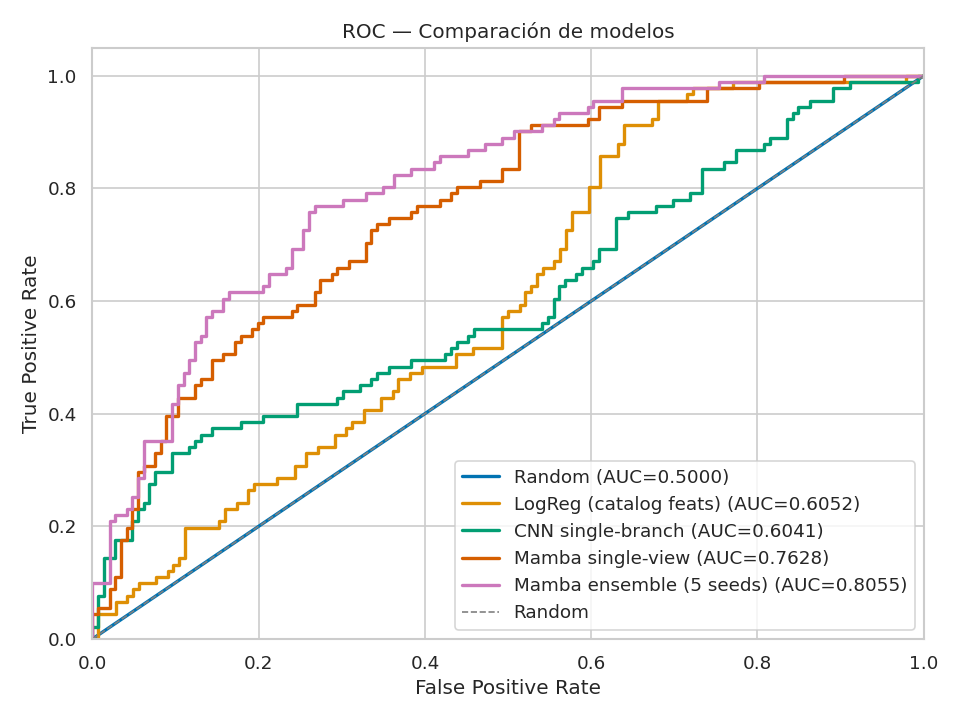
\includegraphics[width=\columnwidth]{figures/roc_tier1.png}
\caption{Test ROC curves for the global-view models. Mamba (upper-left) is clearly
separated from the CNN and logistic regression (near the diagonal); the visual
gap is the $+0.20$ AUC difference quantified in Table~\ref{tab:delong}.}
\label{fig:roc}
\end{figure}

\subsection{Calibration, confusion and error structure}

The Mamba ensemble is also better calibrated (Brier $0.192$ vs.\ $0.271$ for the
CNN; see Fig.~\ref{fig:cal}). Its improvement is qualitative, not just ranking:
relative to the CNN it roughly halves false positives (55 vs.\ 96) and nearly
doubles true negatives (91 vs.\ 50) on the same 237 test stars, i.e.\ it rejects
catalog FPs the CNN accepts. An automated error breakdown (Fig.~\ref{fig:err})
localizes the dominant failure mode: transits with depth $\in(136,770]$\,ppm have a
45.8\% error rate ($n=48$)---shallow transits near the TESS photometric noise
floor. The hardest false positives are eclipsing binaries with deep, symmetric
dips, the known information limit of single-view vetting.

\begin{figure*}[!t]
\centering
\subfloat[Confusion matrix]{
\includegraphics[width=0.45\textwidth]{results/mamba_ensemble/confusion_matrix.png}}
\hfil
\subfloat[Reliability diagram]{
\includegraphics[width=0.45\textwidth]{results/mamba_ensemble/calibration.png}}
\caption{Mamba ensemble on the sealed test set.}
\label{fig:cal}
\end{figure*}

\begin{figure*}[!t]
\centering
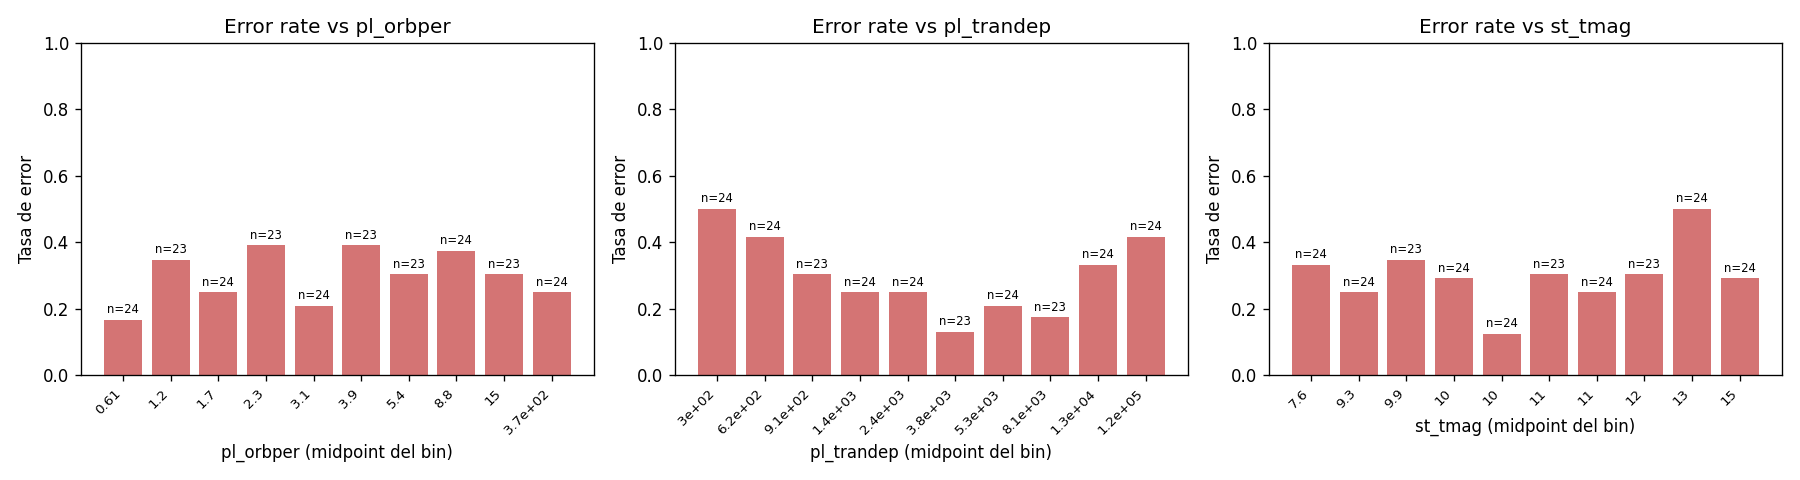
\includegraphics[width=0.95\textwidth]{results/error_analysis/mamba_ensemble/error_rate_by_feature.png}
\caption{Error rate vs.\ binned period, transit depth and stellar magnitude.
Errors concentrate in shallow transits near the noise floor.}
\label{fig:err}
\end{figure*}

\subsection{Explainability}

Applying gradient saliency, integrated gradients~\cite{sundararajan2017} and
occlusion sensitivity to the best Mamba seed over eight confident test cases
(top-2 per TP/TN/FN/FP quadrant), the three methods agree
(Fig.~\ref{fig:xai}): for true positives the attribution concentrates on the
periodic transit dips---the model ``looks in the right place''; for false negatives
it is weak and diffuse; for false positives it correctly fires on real dips but
cannot separate planetary transits from eclipsing binaries, consistent with the
error analysis.

\begin{figure*}[!t]
\centering
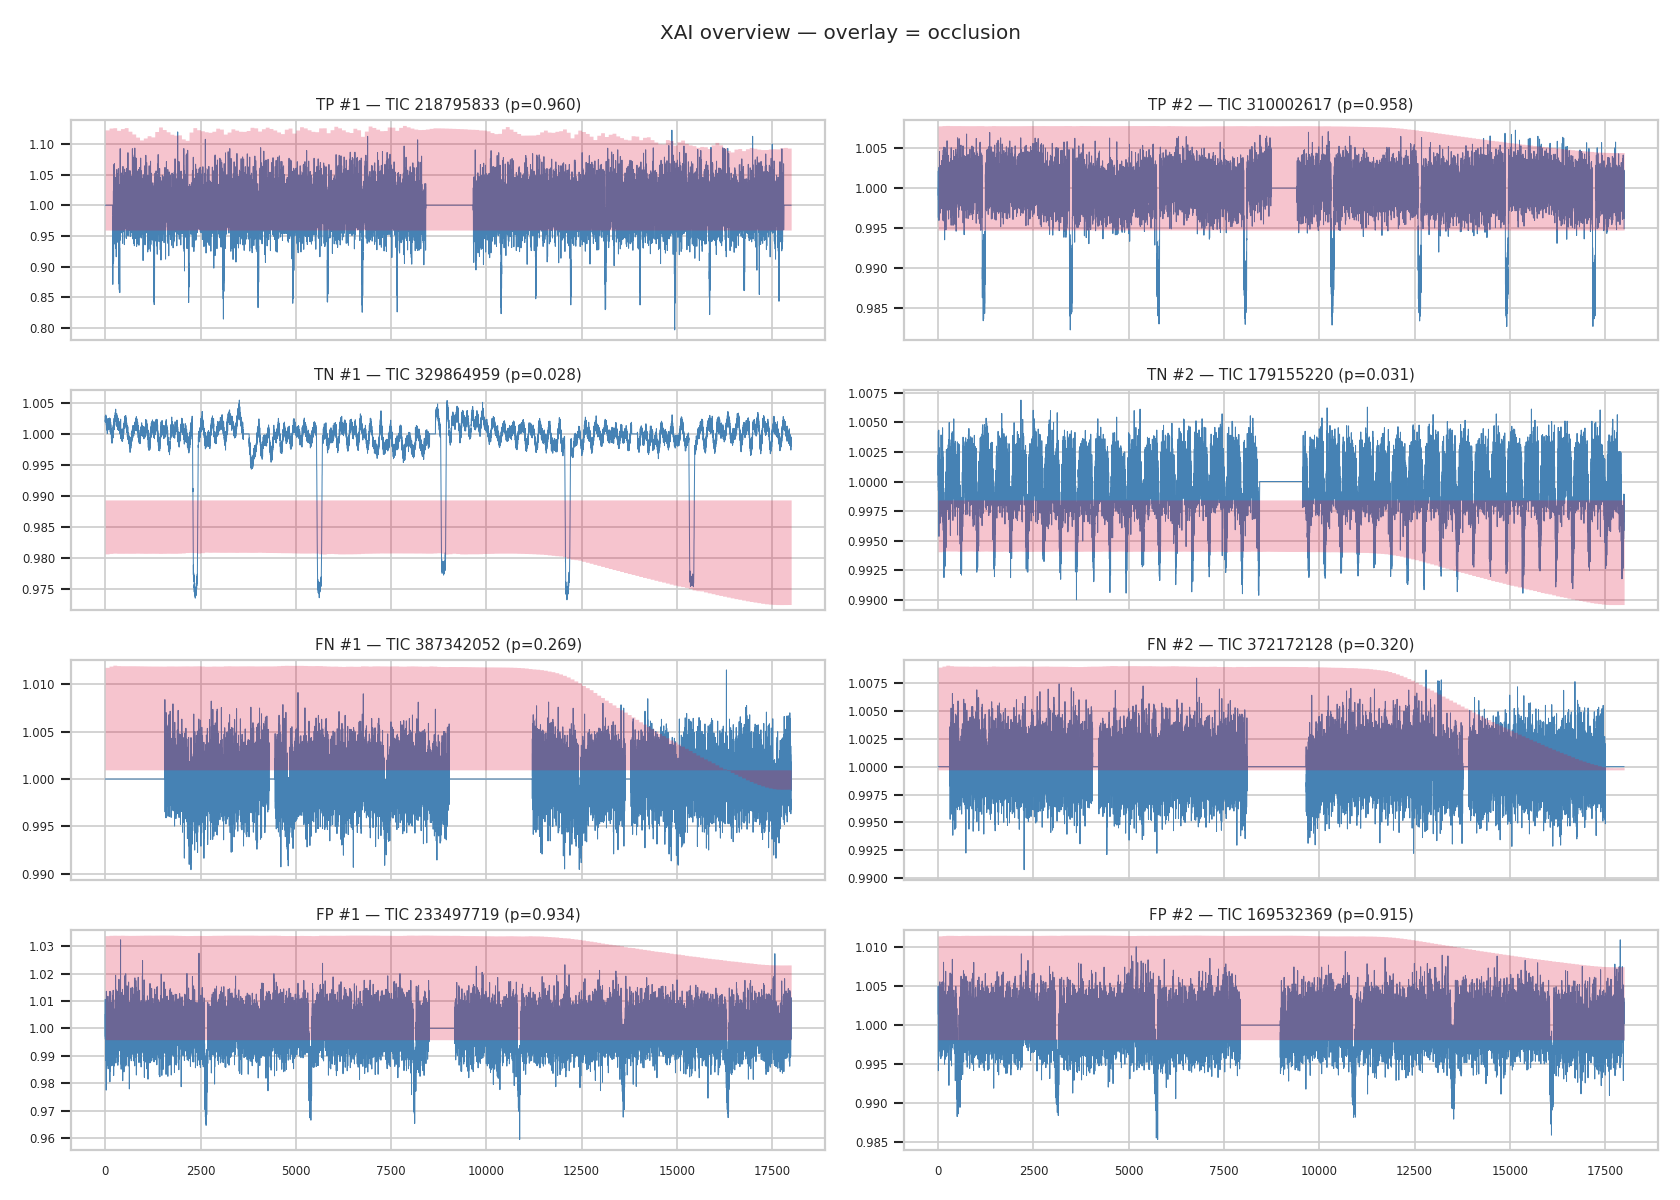
\includegraphics[width=0.88\textwidth]{figures/xai/mamba_seed789/_summary.png}
\caption{Attribution summary (8 cases $\times$ 3 methods) for the best Mamba seed.
Red/blue indicate evidence toward ``planet''/``not planet''. True positives place
mass on the transit dips.}
\label{fig:xai}
\end{figure*}

\subsection{Negative ablation: naive Mamba\,$+$\,CNN late fusion}

ExoMamba V1 (Table~\ref{tab:main}, last row) collapses \emph{below chance}
($0.460$ $[0.382,0.541]$) across three seeds, despite passing a sanity overfit
(val AUC $=1.0$ on 64 examples), ruling out an implementation bug. We read this as
the fusion operator, not the branches, being at fault: a tiny concat-MLP head lets
the fast-training local CNN dominate the gradient and starve the Mamba encoder.
The dual-branch AstroNet, with a $\sim$700K-parameter FC head, instead recovers
the local-view signal ($+0.11$ over the single-branch CNN). The lesson is that
combining selective state-space and convolutional features needs a non-trivial,
jointly trained fusion---naive late concatenation is the wrong operator---which
motivates gated/attention fusion as future work rather than a headline result.

% =============================================================================
\section{Discussion}

The $+0.20$ AUC gap over the CNN is not explained by capacity (Mamba 131K vs.\
CNN 63K, only $2\times$). It is architectural: our single-branch CNN's effective
receptive field ($\sim$80 cadences) cannot see the multi-day periodicity of
transits, while Mamba's $O(L)$ state recursion integrates all transits in a sector
into one latent trajectory. A much larger dual-branch CNN (AstroNet, 1.34M) with an
explicit local view narrows but does not close the gap, and---without
Kepler-to-TESS transfer learning, which the strongest published systems rely
on---underfits this small training set. Taken together, on $\sim$1{.}6K labelled
TOIs and a 4\,GB GPU, long-range sequence modeling of the complete global curve is
the most effective single design choice we tested.

We stress what this does \emph{not} show. It is not a vetting state of the art:
AstroNet/ExoMiner-class systems use far larger datasets, transfer learning and
richer diagnostics. It is a controlled feasibility result: under matched data, a
single sealed split and quantified uncertainty, selective state-space modeling
beats tabular and shallow-convolutional baselines by a margin that survives DeLong
and bootstrap testing.

% =============================================================================
\section{Limitations}

\textbf{Small data.} 1{,}576 labelled TOIs ($\sim$1/10 of Kepler-scale training
sets) is the main constraint; absolute AUC (0.806) is below what large-data,
transfer-learning systems report, as expected. \textbf{Label selection bias.}
We use CP vs.\ FP; confirmed planets tend to be better-studied and cleaner than
the broader, more operationally relevant PC-vs-FP (candidate triage) problem, so
our labels likely make the task somewhat easier and less representative of live
triage. \textbf{No transfer learning} from Kepler (no reliable public checkpoint),
which disadvantages the dual-branch CNN in particular. \textbf{No external
validation} on held-out sectors or an independent catalog, and \textbf{no common
benchmark} against ExoMiner++/DART-Vetter under identical inputs. \textbf{No
$k$-fold CV} (compute-bound), mitigated by multi-seed reporting. These bound the
claim to a within-study, same-split comparison.

% =============================================================================
\section{Conclusion and Future Work}

Under a sealed TIC-level split, matched inputs and quantified uncertainty, a
compact selective state-space model provides a computationally feasible alternative
for modeling long TESS light curves and significantly outperforms tabular and
shallow-convolutional baselines for CP/FP TOI vetting. The result should be
interpreted as a controlled feasibility study rather than a production vetting
catalog. Future work should test non-naive fusion of global SSM features, local
phase-folded views and scalar catalog features; transfer learning from Kepler to
TESS; extension to the operational PC-vs-FP triage setting; and external validation
on independent TOI snapshots or held-out sectors.

\textbf{Reproducibility.} All splits are versioned at the TIC level; every run
stores its config, git commit, environment, training curve, checkpoints and
per-sample test predictions; the test set is loaded once behind an explicit guard;
49 unit tests cover the data and metrics paths. Inference statistics are computed
from the stored predictions by a single script, so all confidence intervals and
DeLong tests in this paper are reproducible without retraining.

\textbf{Code availability.} Code, split files, experiment configurations and stored
prediction files are available at \url{https://github.com/JoseZum/ExoMamba}.

\balance

% =============================================================================
\begin{thebibliography}{00}

\bibitem{gu2023mamba} A.~Gu and T.~Dao, ``Mamba: Linear-Time Sequence Modeling with
Selective State Spaces,'' arXiv:2312.00752, 2023.

\bibitem{shallue2018} C.~J.~Shallue and A.~Vanderburg, ``Identifying Exoplanets with
Deep Learning: A Five-planet Resonant Chain around Kepler-80,'' \emph{Astron. J.},
vol.~155, no.~2, p.~94, 2018.

\bibitem{valizadegan2022} H.~Valizadegan \emph{et al.}, ``ExoMiner: A Highly
Accurate and Explainable Deep Learning Classifier to Mine Exoplanets,''
\emph{Astrophys. J.}, vol.~926, no.~2, p.~120, 2022.

\bibitem{yu2019} L.~Yu \emph{et al.}, ``Identifying Exoplanets with Deep Learning.
III. Automated Triage and Vetting of TESS Candidates,'' \emph{Astron. J.},
vol.~158, no.~1, p.~25, 2019.

\bibitem{exominerpp} H.~Valizadegan \emph{et al.}, ``ExoMiner++ on TESS with
Transfer Learning from Kepler: Transit Classification and Vetting Catalog for
2-min Data,'' arXiv:2502.09790, 2025.

\bibitem{dartvetter} S.~Fiscale \emph{et al.}, ``DART-Vetter: A Deep LeARning Tool
for automatic triage of exoplanet candidates,'' arXiv:2506.05556, 2025.

\bibitem{armstrong2020} D.~J.~Armstrong, J.~Gamper, and T.~Damoulas, ``Exoplanet
Validation with Machine Learning: 50 new validated Kepler planets,''
arXiv:2008.10516, 2020.

\bibitem{sundararajan2017} M.~Sundararajan, A.~Taly, and Q.~Yan, ``Axiomatic
Attribution for Deep Networks,'' in \emph{Proc. Int. Conf. Mach. Learn. (ICML)},
2017.

\bibitem{delong1988} E.~R.~DeLong, D.~M.~DeLong, and D.~L.~Clarke-Pearson,
``Comparing the Areas under Two or More Correlated Receiver Operating
Characteristic Curves,'' \emph{Biometrics}, vol.~44, no.~3, pp.~837--845, 1988.

\bibitem{sun2014} X.~Sun and W.~Xu, ``Fast Implementation of DeLong's Algorithm for
Comparing the Areas Under Correlated Receiver Operating Characteristic Curves,''
\emph{IEEE Signal Process. Lett.}, vol.~21, no.~11, pp.~1389--1393, 2014.

\bibitem{lightkurve} Lightkurve Collaboration, ``Lightkurve: Kepler and TESS time
series analysis in Python,'' Astrophys. Source Code Libr., ascl:1812.013, 2018.

\bibitem{toi} NASA Exoplanet Archive, ``TESS Mission (TOI Catalog).'' [Online].
Available: \url{https://exoplanetarchive.ipac.caltech.edu/docs/TESSMission.html}

\bibitem{mast} MAST Archive, ``TESS Mission Data Archive.'' [Online]. Available:
\url{https://archive.stsci.edu/missions-and-data/tess}

\end{thebibliography}

\end{document}
